\documentclass[11pt]{article}


\usepackage{geometry}
\geometry{letterpaper}


\usepackage{doc}
\usepackage{cite}
\usepackage[margin=1cm]{caption}

\usepackage{url}


\usepackage{graphicx}
\usepackage{epstopdf}
\DeclareGraphicsRule{.tif}{png}{.png}{`convert #1 `dirname #1`/`basename #1 .tif`.png}


\title{A ``Dream'' Interface Design}
\author{Rachel Rivera}
\date{November 25, 2014}


\begin{document}


\maketitle


\begin{abstract}
This investigation purposes a ``dream'' user interface for touch screen devices. 
\end{abstract}


\pagebreak
\tableofcontents



\pagebreak


\section{Introduction}
\label{Introduction}

Mobile devices are ubiquitous in contemporary society. The latest figures from the United Nations' telecommunications agency estimate that there are around 6.8 billion cell-phone subscriptions in the world \cite{UNTelecommunications	}. Thus, the investigation and development of usable interfaces for mobile devices is a significant research topic.

Many mobile devices use touchscreen keyboards instead of physical keyboards. This allows for a larger display without increasing the size of the device. Furthermore, touchscreen keyboards have the ability to change their layout based on user input and disappear when not needed. To compensate for the lack of tactile feedback provided by physical keys, touchscreen keyboards often include aural feedback in the form of audible clicks from a speaker. Haptic feedback in the form of device vibrations is often included as well.

Even with these alternate forms of feedback, the literature suggests that insufficient feedback is still a major usability issue with touchscreen mobile devices. \cite{Tinwala:2010:ETE:18	68914.1868972, Kane:2011:UGB:1978942.1979001, Hardy:2008:TIT:1409240.1409267, El-Glaly:2013:TTF:2460625.2460665, Buxton:1986:HID:22339.22386}. A study by Hussain Tinwala and Scott MacKenzie submits that the lack of physical keys requires heightened visual attention from the user, which diverts the user's concentration from the thoughts being expressed \cite{Tinwala:2010:ETE:18 68914.1868972}. The lack of physical keys not only diverts the attention of some users, but it also makes the device  almost entirely unusable for other users. A study from Virginia Polytechnic Institute and State University demonstrates how touchscreen mobile devices do not provide sufficient feedback for Individuals with Blindness or Severe Visual Impairment (IBSVI) as these users are only able to ``develop a spatial mental model for the interface or the screen through dead reckoning'' \cite{El-Glaly:2013:TTF:2460625.2460665}. 

Thus, the aim of this investigation is to propose a ``dream'' interface design that addresses some of these usability issues.


\section{System Description}
\label{System Description}

In this investigation, I propose a ``dream'' interface design for touchscreen mobile devices that provides a significant amount of tactile feedback. This feedback is designed in a way that can be helpful for individuals with and without visual impairments alike. This design was developed with the usability metrics of learnability, efficiency, and errors in mind.

This design makes use of technology that is currently being created by Tactus, a company in Fremont California \cite{Tactus}. Tactus brings real physical buttons that dynamically appear and disappear into a flat touch screen (see Figure~\ref{tactus}). Small fluid channels are routed throughout the Tactile Layer and enable fluid ot expand the top polymer layer to create the physical buttons \cite{Tactus}.

Although this technology from Tactus is extremely bleeding-edge, it has already received a fair amount of recognition \cite{CNN, I-Zone, PCMag}. 

\begin{figure}[ht]
\centering
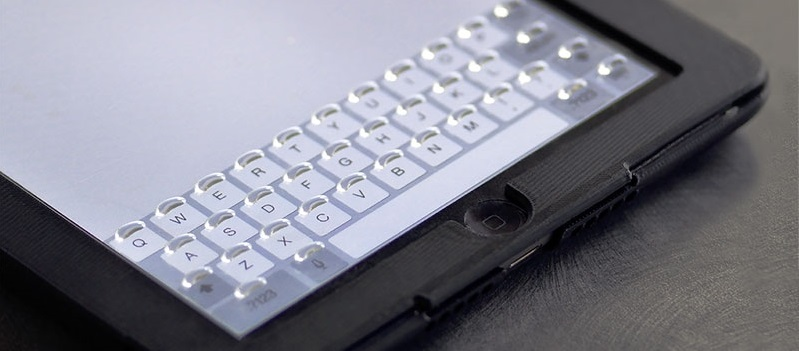
\includegraphics[width=4.5in]{tactus1.jpg} 
\caption{Tactus Technology keyboard}
\label{tactus}
\end{figure}

\section{Top-Level Design}
The design aims to assist IBSVI engage their spatial cognition, perception and sensing resources while interacting with touch screens. The tactile stuff is intended to operate in conjunction with other technologies that provide auditory feedback that informs the users of \textit{what} is at the location on the screen while the tactile buttons heps the user know \textit{where} it is. 
\label{background}

\section{Usage Scenarios}

\section{Rationale}


\section{Usability Metric ``Forecast''}
\clearpage


\bibliography{mybib}{}
\bibliographystyle{plain}
\end{document}

\end{document}
	